
\documentclass{beamer}
\usepackage[utf8]{inputenc}
\usepackage{graphicx}
\usepackage{wrapfig}
\usepackage{xcolor}






\usetheme{Madrid}

\AtBeginSection[]{
	\begin{frame}
		\vfill
		\centering
		\begin{beamercolorbox}[sep=8pt,center,shadow=true,rounded=true]{title}
			\usebeamerfont{title}\insertsectionhead\par%
		\end{beamercolorbox}
		\vfill
	\end{frame}
}

\title{Replication Study: Machine Labor (Angrist, 2022)}
\subtitle {Research Module Econometrics}
\author{Cristian Gutierrez, Marcel Wachter}
\centering
\date{January 14, 2023}
\begin{document}
\maketitle

\begin{frame}
\frametitle{Overview} 

\begin{itemize}
    

\item Main idea of Angrist (2022)
\item Motivation
\item Theory
\item Replication Study
\item Conclusion
\end{itemize}
\end{frame}


\begin{frame} {Main idea of Angrist (2022)}
\begin{itemize}
\item  Angrist (2022) studies utility of machine learning (ML) algorithms for regression-based causal inference using lasso to select control variables for estimates of college characteristics' wage effect.
\end{itemize}

\end{frame}






\begin{frame}{Motivation}
\begin{itemize}
    \item Angrist (2022): Selecting the correct controls from a dictionary allows to make valid inference.
\end{itemize}
\includegraphics[width=0.4\textwidth]{Table 1 Angrist (2022).png}
\end{frame}


\begin{frame}{Theory}
\begin{flushleft}
\item Consider a standard linear regression model. 
\end{flushleft}
\[
    y_i=\boldsymbol{\beta_0} +\mathbf{x}_i^\prime \boldsymbol{\beta}+\epsilon_i, \quad i = 1, \ldots, n,
    \tag{1}
\]
\begin{flushleft}
It's estimator looks as follows
\end{flushleft}
\[
\hat{\boldsymbol{\beta}}^{\text{OLS}}=\underset{\boldsymbol{\beta}}{\arg \min}\sum_{i=1}^N (y_i-\beta_0-\sum_{j=1}^k x_{i j}\beta_j)^2
    \tag{2}
\]
\begin{flushleft}
where $\mathbf{x}_i=(x_{i1}, ..., x_{ik})$ and $k$ is the number of regressors.
\end{flushleft}
\end{frame}


\begin{frame}{Theory: Lasso}
\begin{flushleft}
LASSO expands the OLS minimand in equation (2) by adding a regularization term  
that favors smaller coefficients and lower-dimensional models over an unrestricted OLS fit.

Formally, 
\end{flushleft}
	\[
	\hat{\boldsymbol{\beta}}^{\text{LASSO}} =\underset{\boldsymbol{\beta}}{\arg \min}\left\{\frac{1}{2}\sum_{i=1}^N (y_i-\beta_0-\sum_{j=1}^k x_{i j}\beta_j)^2 +\lambda \left(\sum_{j=1}^k |\beta_j|\right)\right\}
	\tag{3}
	\]

\begin{flushleft}
Note: Lasso is contructed upon the assumption of \textbf{approximate sparsity} that consists of only a small subset of covariates, $s^2<<n$ taking non-zero values, where $s$ represents
a sparse vector explainin the outcome and n the number of observations.
\end{flushleft}
\end{frame}


\begin{frame}{Theory: The penalty term $\lambda$}
	\begin{flushleft}
	In contemporary Machine Learning the penalty term is chosen by Cross-Validation. However, 
	Belloni et al. (2012,2014b) proposes an alternative data-driven procedure as follows:
	\[
	\lambda=2c \sqrt{n} \phi^{-1} (\frac{1-\gamma}{2p})
		\tag{4}
	\]
	where $c>1$ is a constant, $(1-\gamma)$ a confidence interval, $k$ the number of regressors and $\phi$ the cummulative standard normal distribution
	accoring to Belloni et al (2014b).
	\end{flushleft}
\end{frame}


\begin{frame}{Theory: Testing Lasso features}
\begin{flushleft}
This section shows various simulations that intend to test the approximate sparsity assumption of LASSO.
\end{flushleft}
	\begin{itemize}
		\item The data generating process is as follows:
		\[Y_i = \beta X_i + \varepsilon_i\]
		with \(X_i \stackrel{iid}{\sim} \mathcal{N}(0_p,I_p)\), \(\varepsilon_i \stackrel{iid}{\sim} \mathcal{N}(0,1)\), and \(\beta  {\sim}  \mathcal{U}(0.1,0.5)\) 
	\end{itemize}
\end{frame}


\begin{frame}{Theory: Testing Lasso features}
	\begin{itemize}
		\item Attach here the following results: Increasing sparsity
	\end{itemize}
\end{frame}



\begin{frame}{Theory: Testing Lasso features}
	\begin{itemize}
		\item Attach here the following results: High-dimensional scenario Lasso vs Rigorous Lasso
	\end{itemize}
\end{frame}


\begin{frame}{Replication Study}
\begin{itemize}
  
\item **Text** \textbf{**Text**}.
\item **Text**. 
\item **Text** .
\end{itemize}

\includegraphics[width=0.4\textwidth]{/Users/marcel/Uni/MSc/3rd/RM_Econometrics/project/rm_econometrics/Presentation/Table 1 Angrist (2022).png}
\end{frame}

\begin{frame}{Theory: Post Double Selection}
Consider the simple linear model
\[Y_i = \alpha D_i + \beta X_i + \varepsilon_i\]
\[D_i = \delta X_i + \upsilon_i\]
with \(X_i \stackrel{iid}{\sim} \mathcal{N}(0_p,I_p)\), \(\varepsilon_i \stackrel{iid}{\sim} \mathcal{N}(0,1)\), and \(\upsilon_i \stackrel{iid}{\sim} \mathcal{N}(0,1)\) 
\end{frame}

\begin{frame}{Simulation: Inference with Selection among Many Controls}
	
\end{frame}



\begin{frame} {Conclusions}
\begin{itemize}
\item Data-driven penalties do not improve prediction performance but may ease model interpretation under high sparsity scenarios.
\item Lasso improves the process of feature selection in Labor Economics under approximate sparsity.  
\item ML learning algorithms seem  ill-suited for IV applications in Labor Economics.
\end{itemize}
\end{frame}

\end{document}
